\documentclass[border=8pt]{standalone}
\usepackage{amsmath,amssymb}
\usepackage{tikz}
\begin{document}
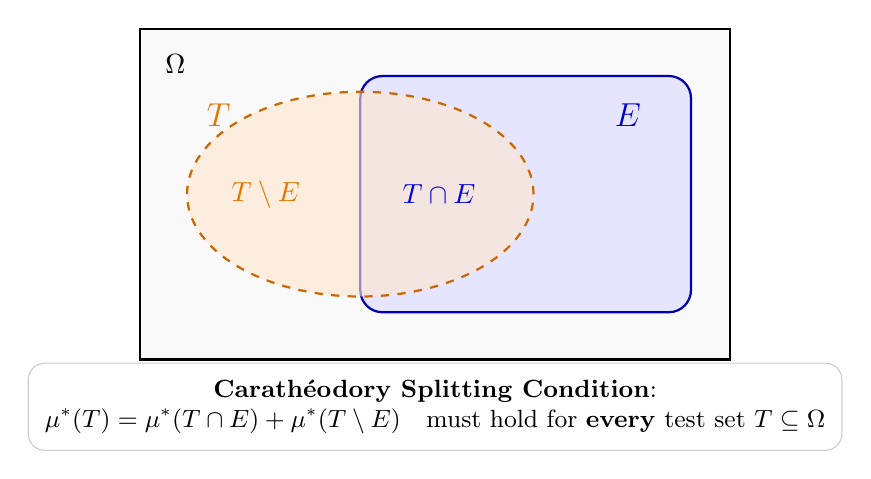
\begin{tikzpicture}[font=\small]
  % Space Omega
  \draw[thick, fill=gray!5] (0, 0) rectangle (7.5, 4.2);
  \node[anchor=north west, font=\bfseries] at (0.2, 4.0) {$\Omega$};

  % Candidate measurable set E
  \draw[thick, fill=blue!10, draw=blue!70!black, rounded corners=8pt] (2.8, 0.6) rectangle (7.0, 3.6);
  \node[font=\bfseries\large, text=blue!80!black] at (6.2, 3.1) {$E$};

  % Test set T (ellipse crossing the boundary of E)
  \draw[thick, dashed, fill=orange!20, draw=orange!80!black, fill opacity=0.6] (2.8, 2.1) ellipse (2.2cm and 1.3cm);
  \node[font=\bfseries\large, orange!90!black] at (1.0, 3.1) {$T$};

  % Intersection T \cap E and difference T \setminus E
  \node[align=center, font=\bfseries, text=blue!90!black] at (3.8, 2.1) {$T \cap E$};
  \node[align=center, font=\bfseries, text=orange!90!black] at (1.6, 2.1) {$T \setminus E$};

  \node[align=center, fill=white, draw=gray!40, rounded corners=6pt, inner sep=6pt] at (3.75, -0.6)
    {\textbf{Carathéodory Splitting Condition}:\\
     $\mu^*(T) = \mu^*(T \cap E) + \mu^*(T \setminus E) \quad \text{must hold for \textbf{every} test set } T \subseteq \Omega$};
\end{tikzpicture}
\end{document}
